\chapter{Implementation}
\label{cha:implementation}

For the implementation of our algorithm, we use the distributed framework Apache Spark\footnote{http://spark.apache.org/}. In this chapter, we will firstly introduce some knowledge about spark and how we use these techniques to implement our model. After that, we will introduce the experiments we did and analysis our results.


\section{Introduction of Spark}


Spark was developed by \cite{ZahariaChowdhuryEtAl2010} and has many useful features for the parallel execution of programs. As the basic datastructure it has the 
\gls{RDD} % RDD
(Resilient Distributed Dataset). The RDD is a special data structure containing the items of a dataset, e.g. sentences or documents. Spark automatically distributes these items over a cluster of compute nodes and manages its physical storage. 

Spark has one driver and several executors. Usually, an executor is a cpu core, and we call each machine as worker, so each worker has several executors. But logically we only need the driver and the executors, only for something about tuning we should care about the worker stuff, e.g. some operations need to do communication between different machine. But for most of cases, each executor just fetches part of data and deals with it, and then the driver collects data from all executors.

The Spark operations can be called from different programming languages, e.g. Python, Scala, Java, and R. For this thesis we use Scala to control the execution of Spark and to define its operations.

Firstly, Spark reads text file from file system (e.g. from the unix file system or from HDFS, the Hadoop file system) and creates an RDD. An RDD usually is located in the RAM storage of the different executors, but it may also stored on (persisted to) disks of the executors. Spark operations follow the functional programming approach. There are two types of operations on RDDs: \emph{Transformation operations} and \emph{action operations}.  A transformation operation transforms  a RDD to another RDD. Examples of transformation operations are map (apply a function to all RDD elements), filter (select a subset of RDD elements by some criterion), or sort (sort the RDD items by some key). Note that an RDD is not mutable, i.e. cannot be changed. If its element are changed a new RDD is created. 

Generally after some transformation operations, people use action operations to gain some useful information from the RDD. Examples of action operations are count (count the number of items), reduce (apply a single summation-like function), aggregate (apply several summation-like functions), and collect (convert an RDD to a local array). 
 


\section{Implementation}

We use $syn0$ to represent the input embedding $V$ and $syn1$ to represent the output embedding $U$. $syn0$ and $syn1$ are defined as broadcast variables, which are only readable and can not be changed by executors. When they are changed in a training step copies are returned as a new RDD.


\paragraph{Data preparing} 
We use the same corpus as other papers used, a snapshot of Wikipedia at April, 2010 created by \cite{Shaoul2010}, which has 990 million tokens. Firstly we count the all words in the corpus. We transform all words to lower capital and then generate our vocabulary (dictionary). And then we calculate the frequency of word count. For example, there are 300 words which appear 10 times in the corpus. So the frequency of count 10 is 300. From this we can calculate the accumulated frequency. That is, if the accumulated frequency of count 200 is 100000, there would be 100000 words whose count is at least 200. This accumulated frequency can be used to select a vocabulary $D$ with the desired number of entries, which all appear more frequent than $minCount$ times in the corpus.  If the count of a word is smaller than $minCount$ we remove it from corpus, so it won't be in the vocabulary.  

\begin{figure}[H]
\centering
\begin{minipage}{.5\textwidth}
 
        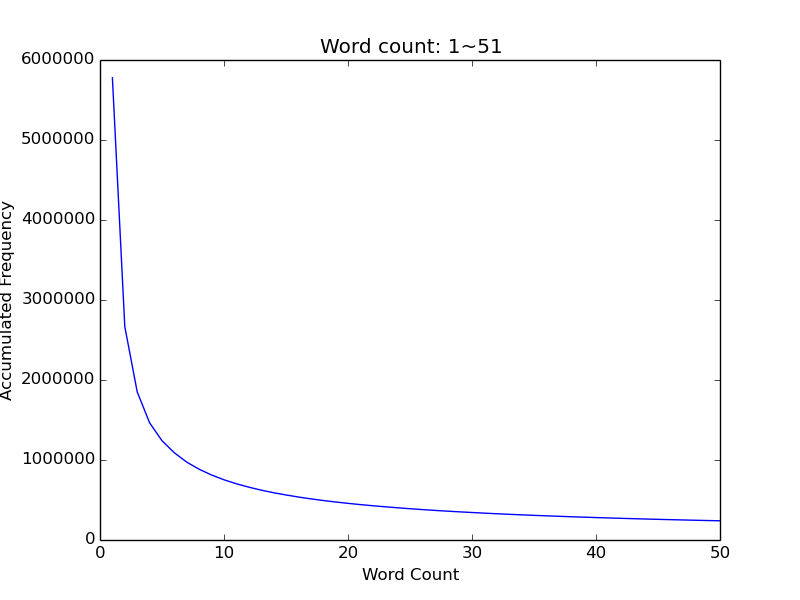
\includegraphics[width=1.0\textwidth]{1to51} 
	\caption{1to51}
	\label{fig:1to51}
\end{minipage}%
\begin{minipage}{.5\textwidth}
  
        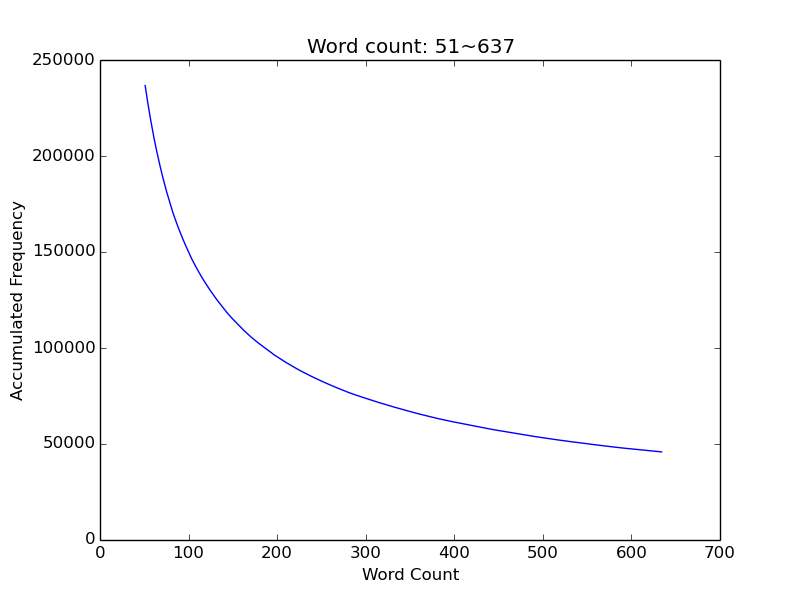
\includegraphics[width=1.0\textwidth]{51to637} 
	\caption{51to637}
	\label{fig:51to637}
\end{minipage}
\end{figure}


\begin{figure}[H]
\centering
\begin{minipage}{.5\textwidth}
 	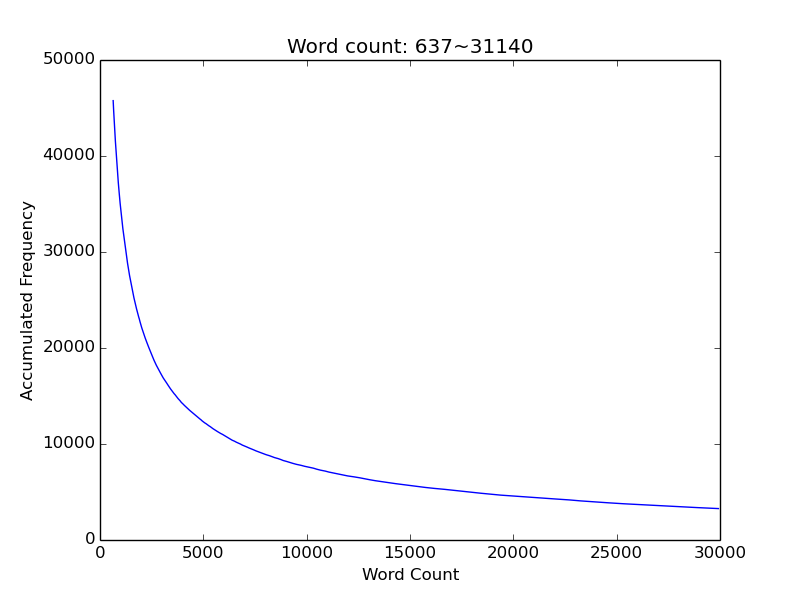
\includegraphics[width=1.0\textwidth]{637to31140} 
	\caption{637to31140}
	\label{fig:637to31140}
\end{minipage}%
\begin{minipage}{.5\textwidth}
	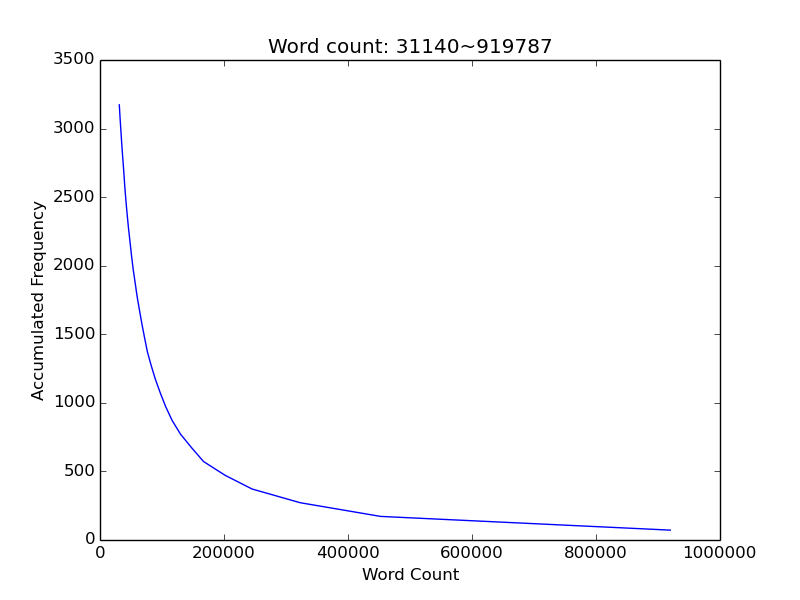
\includegraphics[width=1.0\textwidth]{31140torest} 
	\caption{31140torest}
	\label{fig:31140torest}
\end{minipage}
\end{figure}

\paragraph{Computing Environment} \ \\
Our program is running on a single machine with 32 cores. For some experiments, we use all cores as executers. We also tried some experiments on a compute cluster of several machines, but that is not very good for our program, we will explain some reasons later. So there is no communication between different machines.  But there are some experiments requiring fewer cores.


\paragraph{Training set and validation set} \ \\
We split the corpus into a training set and a validation set. The training set has $99\%$ of the data and validation set has only $1\%$ of the data. We use the validation set to monitor our training process if it is converging. If the training algorithm  converges, the loss of validation set should be at the lowest value. And then it will gradually increase, which means the training is over-fitting. So we will calculate the loss of the validation set after several training iterations and then compare with the previous validation loss. If the current value is bigger than previous value, we stop our training process and fetch the previous result as the final result to store to the disk. That is, after each calculation of the loss of validation set, we will store our results. 

Note that, because we want to use the validation set to monitor our training, the validation set and training set should not be overlapping. And another import thing is that, the negative samples of validation set should always be fixed to reduce variance.  The assignment step for the word senses of the validation set is almost the same as the one for training set. The only different thing is that the negative samples for each word of each sentence in the validation set are not changed. But for each iteration of sense assignment for sentences in the training set, the negative sampling are new. 

\paragraph{Assign Step}\ \\
In the assignment, we use map transformation to transform each sentence with senses information to another sentence with changed senses information. The sense with the lowes loss is selected. So one RDD is transformed to another RDD. In this process, $syn0$ and $syn1$ are constant and will be used (only read) to calculate the loss. 

\paragraph{Learn Step}\ \\
In the training, we also use a map transformation. Instead of transforming sentences to sentences, we transform the original sentence RDD into the two-element collection of the updated $syn0$ and updated $syn1$. We broadcast these variables to the local $syn0$ and $syn1$ in each executor, so that each executor has its own  copy of $syn0$ and $syn1$ and can update them independently. So each executor has copies of $syn0$ and $syn1$. And then we use $treeAggregate$ to collect all such vectors together from different executors (cpu cores).  In the aggregation operation, different $syn0$'s vectors add up together, and different $syn0$'s vectors add up together. Finally, by dividing by the the number of partitions, we get one global $syn0$ and one global $syn1$ in the driver. For now, we set them as new $syn0$ and $syn1$, which will be broadcasted again in the next iteration. 

\paragraph{Normalization}\ \\
After getting the new global $syn0$ and $syn1$, some values of some embeddings may be very big. Thus, we need to do normalization to avoid to big values. Our normalization method is very simple, which is to check all embeddings from $syn0$ and $syn1$ if their Euclidean length is bigger than 4. If that is the case we just normalize them to the new embeddings with length of 4.






